We remind that the end of the algorithm, using matrix approximation to compute the filtered image, is not implemented.
Nonetheless, we will present interesting results about the computation of the eigenvalues of the graph Laplacian operator.
We consider a picture with 402 318 pixels and we sample 1\% of them, which corresponds approximately to 4000 sample pixels.
Additionally to varying the number of processors, we also vary the number of computed eigenvalues from 50 up to 500.
Here are the first 500 eigenvalues of the Laplacian submatrix:

\begin{figure}[H]
  \centering
  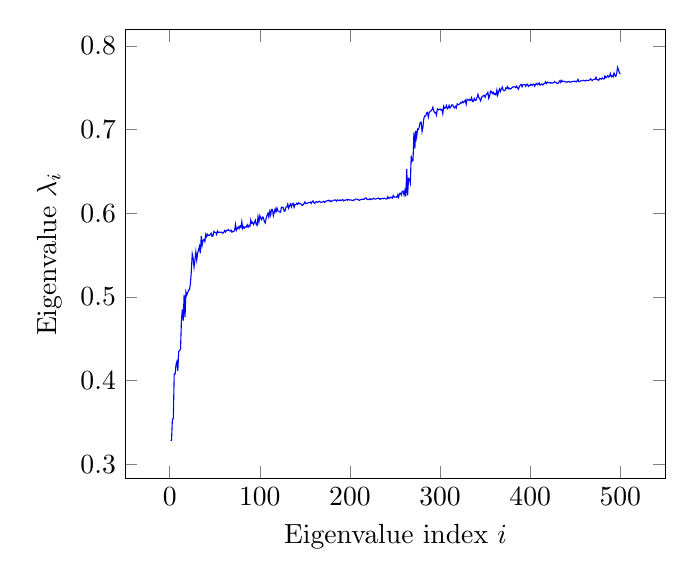
\begin{tikzpicture}
 \begin{axis}[
  xlabel=Eigenvalue index \(i\),
  ylabel=Eigenvalue \(\lambda_i\)]
  \addplot[color=blue] coordinates {
   (1, 0.328403)
   (2, 0.328993)
   (3, 0.354142)
   (4, 0.354558)
   (5, 0.407947)
   (6, 0.407922)
   (7, 0.419087)
   (8, 0.422894)
   (9, 0.411912)
   (10, 0.434953)
   (11, 0.436195)
   (12, 0.437591)
   (13, 0.471408)
   (14, 0.485145)
   (15, 0.471876)
   (16, 0.50277)
   (17, 0.47612)
   (18, 0.506129)
   (19, 0.50255)
   (20, 0.505246)
   (21, 0.508385)
   (22, 0.508875)
   (23, 0.516208)
   (24, 0.530951)
   (25, 0.551366)
   (26, 0.546031)
   (27, 0.535797)
   (28, 0.54417)
   (29, 0.553869)
   (30, 0.544179)
   (31, 0.552599)
   (32, 0.556183)
   (33, 0.560408)
   (34, 0.552089)
   (35, 0.57255)
   (36, 0.561992)
   (37, 0.567683)
   (38, 0.568707)
   (39, 0.566264)
   (40, 0.575036)
   (41, 0.572075)
   (42, 0.574888)
   (43, 0.573638)
   (44, 0.573606)
   (45, 0.574707)
   (46, 0.576157)
   (47, 0.572465)
   (48, 0.572887)
   (49, 0.578266)
   (50, 0.577289)
   (51, 0.577101)
   (52, 0.574753)
   (53, 0.578846)
   (54, 0.577053)
   (55, 0.577171)
   (56, 0.577384)
   (57, 0.577616)
   (58, 0.577029)
   (59, 0.576138)
   (60, 0.577424)
   (61, 0.579389)
   (62, 0.577662)
   (63, 0.579514)
   (64, 0.579413)
   (65, 0.580647)
   (66, 0.579368)
   (67, 0.578908)
   (68, 0.579853)
   (69, 0.577481)
   (70, 0.57841)
   (71, 0.57815)
   (72, 0.579599)
   (73, 0.586778)
   (74, 0.579563)
   (75, 0.581868)
   (76, 0.583686)
   (77, 0.581725)
   (78, 0.584791)
   (79, 0.58317)
   (80, 0.590067)
   (81, 0.58162)
   (82, 0.58403)
   (83, 0.582365)
   (84, 0.583794)
   (85, 0.58359)
   (86, 0.586169)
   (87, 0.583282)
   (88, 0.585467)
   (89, 0.584366)
   (90, 0.592158)
   (91, 0.587962)
   (92, 0.589138)
   (93, 0.586626)
   (94, 0.589144)
   (95, 0.591788)
   (96, 0.586469)
   (97, 0.585384)
   (98, 0.595982)
   (99, 0.589712)
   (100, 0.597098)
   (101, 0.593938)
   (102, 0.59224)
   (103, 0.595483)
   (104, 0.594726)
   (105, 0.59026)
   (106, 0.588475)
   (107, 0.593881)
   (108, 0.597248)
   (109, 0.600065)
   (110, 0.595491)
   (111, 0.60219)
   (112, 0.597753)
   (113, 0.604718)
   (114, 0.604648)
   (115, 0.597022)
   (116, 0.601191)
   (117, 0.605243)
   (118, 0.601688)
   (119, 0.606338)
   (120, 0.602887)
   (121, 0.602497)
   (122, 0.601607)
   (123, 0.601351)
   (124, 0.60732)
   (125, 0.606745)
   (126, 0.606653)
   (127, 0.602445)
   (128, 0.602744)
   (129, 0.607308)
   (130, 0.607352)
   (131, 0.610958)
   (132, 0.606089)
   (133, 0.609026)
   (134, 0.611262)
   (135, 0.607655)
   (136, 0.611064)
   (137, 0.611929)
   (138, 0.607066)
   (139, 0.610522)
   (140, 0.610409)
   (141, 0.611942)
   (142, 0.610808)
   (143, 0.612479)
   (144, 0.611327)
   (145, 0.611731)
   (146, 0.610665)
   (147, 0.609294)
   (148, 0.609987)
   (149, 0.611622)
   (150, 0.613529)
   (151, 0.611501)
   (152, 0.611571)
   (153, 0.612294)
   (154, 0.612613)
   (155, 0.612933)
   (156, 0.613407)
   (157, 0.611578)
   (158, 0.613732)
   (159, 0.614805)
   (160, 0.612629)
   (161, 0.61192)
   (162, 0.61353)
   (163, 0.613907)
   (164, 0.613104)
   (165, 0.613565)
   (166, 0.614426)
   (167, 0.613664)
   (168, 0.613054)
   (169, 0.613152)
   (170, 0.613743)
   (171, 0.614392)
   (172, 0.613066)
   (173, 0.614177)
   (174, 0.614879)
   (175, 0.614939)
   (176, 0.61559)
   (177, 0.614663)
   (178, 0.615456)
   (179, 0.613848)
   (180, 0.614737)
   (181, 0.614914)
   (182, 0.615532)
   (183, 0.616009)
   (184, 0.615817)
   (185, 0.614419)
   (186, 0.615941)
   (187, 0.615559)
   (188, 0.615346)
   (189, 0.61598)
   (190, 0.615062)
   (191, 0.615785)
   (192, 0.616532)
   (193, 0.614875)
   (194, 0.615483)
   (195, 0.615767)
   (196, 0.61628)
   (197, 0.615569)
   (198, 0.616636)
   (199, 0.616125)
   (200, 0.615727)
   (201, 0.616041)
   (202, 0.615556)
   (203, 0.615182)
   (204, 0.615932)
   (205, 0.615761)
   (206, 0.616798)
   (207, 0.616999)
   (208, 0.616871)
   (209, 0.616434)
   (210, 0.615357)
   (211, 0.61592)
   (212, 0.616345)
   (213, 0.616586)
   (214, 0.616894)
   (215, 0.616613)
   (216, 0.616905)
   (217, 0.618205)
   (218, 0.618257)
   (219, 0.616599)
   (220, 0.616334)
   (221, 0.616325)
   (222, 0.617383)
   (223, 0.616319)
   (224, 0.617059)
   (225, 0.617017)
   (226, 0.617999)
   (227, 0.617267)
   (228, 0.616927)
   (229, 0.617276)
   (230, 0.617597)
   (231, 0.617804)
   (232, 0.618269)
   (233, 0.616643)
   (234, 0.617436)
   (235, 0.617211)
   (236, 0.617794)
   (237, 0.617264)
   (238, 0.618154)
   (239, 0.617462)
   (240, 0.617177)
   (241, 0.617079)
   (242, 0.619852)
   (243, 0.617906)
   (244, 0.618103)
   (245, 0.619186)
   (246, 0.619102)
   (247, 0.61813)
   (248, 0.621239)
   (249, 0.619201)
   (250, 0.619493)
   (251, 0.619594)
   (252, 0.61895)
   (253, 0.621864)
   (254, 0.619021)
   (255, 0.623788)
   (256, 0.623924)
   (257, 0.621764)
   (258, 0.626421)
   (259, 0.626401)
   (260, 0.621975)
   (261, 0.627299)
   (262, 0.620112)
   (263, 0.652731)
   (264, 0.621314)
   (265, 0.641508)
   (266, 0.640666)
   (267, 0.636291)
   (268, 0.66886)
   (269, 0.662238)
   (270, 0.663165)
   (271, 0.696515)
   (272, 0.677108)
   (273, 0.69828)
   (274, 0.690668)
   (275, 0.700609)
   (276, 0.700017)
   (277, 0.703813)
   (278, 0.708642)
   (279, 0.70895)
   (280, 0.697594)
   (281, 0.702937)
   (282, 0.713406)
   (283, 0.716234)
   (284, 0.716115)
   (285, 0.7198)
   (286, 0.720496)
   (287, 0.714957)
   (288, 0.720204)
   (289, 0.721803)
   (290, 0.722229)
   (291, 0.723694)
   (292, 0.72654)
   (293, 0.722341)
   (294, 0.720151)
   (295, 0.720461)
   (296, 0.71714)
   (297, 0.724678)
   (298, 0.723453)
   (299, 0.723952)
   (300, 0.724578)
   (301, 0.723302)
   (302, 0.724001)
   (303, 0.718818)
   (304, 0.727797)
   (305, 0.725351)
   (306, 0.725868)
   (307, 0.72881)
   (308, 0.7249)
   (309, 0.725978)
   (310, 0.728913)
   (311, 0.725651)
   (312, 0.726962)
   (313, 0.729484)
   (314, 0.729512)
   (315, 0.7271)
   (316, 0.725885)
   (317, 0.727652)
   (318, 0.725808)
   (319, 0.730581)
   (320, 0.729557)
   (321, 0.73004)
   (322, 0.730756)
   (323, 0.732401)
   (324, 0.731684)
   (325, 0.733546)
   (326, 0.73228)
   (327, 0.73343)
   (328, 0.735144)
   (329, 0.730156)
   (330, 0.736182)
   (331, 0.735642)
   (332, 0.734628)
   (333, 0.736054)
   (334, 0.734991)
   (335, 0.73812)
   (336, 0.733373)
   (337, 0.733805)
   (338, 0.737036)
   (339, 0.734852)
   (340, 0.735032)
   (341, 0.738114)
   (342, 0.742074)
   (343, 0.738399)
   (344, 0.736564)
   (345, 0.734353)
   (346, 0.738659)
   (347, 0.739091)
   (348, 0.740611)
   (349, 0.740995)
   (350, 0.738616)
   (351, 0.741615)
   (352, 0.742678)
   (353, 0.744339)
   (354, 0.737261)
   (355, 0.739999)
   (356, 0.745976)
   (357, 0.74539)
   (358, 0.743067)
   (359, 0.74462)
   (360, 0.741842)
   (361, 0.742852)
   (362, 0.741281)
   (363, 0.747162)
   (364, 0.741006)
   (365, 0.74558)
   (366, 0.748506)
   (367, 0.745377)
   (368, 0.748645)
   (369, 0.75072)
   (370, 0.747139)
   (371, 0.746351)
   (372, 0.746547)
   (373, 0.749818)
   (374, 0.748981)
   (375, 0.75129)
   (376, 0.748655)
   (377, 0.749352)
   (378, 0.748317)
   (379, 0.749113)
   (380, 0.750187)
   (381, 0.751118)
   (382, 0.750899)
   (383, 0.75122)
   (384, 0.750024)
   (385, 0.751781)
   (386, 0.749717)
   (387, 0.748168)
   (388, 0.751288)
   (389, 0.7532)
   (390, 0.753793)
   (391, 0.750979)
   (392, 0.753583)
   (393, 0.753691)
   (394, 0.75375)
   (395, 0.751578)
   (396, 0.753477)
   (397, 0.754161)
   (398, 0.751536)
   (399, 0.752857)
   (400, 0.752527)
   (401, 0.754162)
   (402, 0.7529)
   (403, 0.753956)
   (404, 0.754121)
   (405, 0.751759)
   (406, 0.754159)
   (407, 0.755096)
   (408, 0.753618)
   (409, 0.754439)
   (410, 0.755523)
   (411, 0.753051)
   (412, 0.753854)
   (413, 0.754381)
   (414, 0.753288)
   (415, 0.75462)
   (416, 0.754951)
   (417, 0.756929)
   (418, 0.754855)
   (419, 0.756627)
   (420, 0.756008)
   (421, 0.755664)
   (422, 0.756235)
   (423, 0.755252)
   (424, 0.755887)
   (425, 0.755456)
   (426, 0.756151)
   (427, 0.757361)
   (428, 0.756083)
   (429, 0.755992)
   (430, 0.755037)
   (431, 0.755263)
   (432, 0.756811)
   (433, 0.758444)
   (434, 0.756257)
   (435, 0.758722)
   (436, 0.757174)
   (437, 0.757314)
   (438, 0.757707)
   (439, 0.756797)
   (440, 0.756883)
   (441, 0.756531)
   (442, 0.757291)
   (443, 0.757449)
   (444, 0.756491)
   (445, 0.756641)
   (446, 0.757202)
   (447, 0.757592)
   (448, 0.757287)
   (449, 0.757687)
   (450, 0.757621)
   (451, 0.756988)
   (452, 0.757984)
   (453, 0.759911)
   (454, 0.757089)
   (455, 0.757452)
   (456, 0.758165)
   (457, 0.758075)
   (458, 0.75864)
   (459, 0.758848)
   (460, 0.758345)
   (461, 0.757997)
   (462, 0.758895)
   (463, 0.758766)
   (464, 0.758405)
   (465, 0.758796)
   (466, 0.759189)
   (467, 0.760668)
   (468, 0.759334)
   (469, 0.758513)
   (470, 0.759774)
   (471, 0.759898)
   (472, 0.759872)
   (473, 0.762496)
   (474, 0.759706)
   (475, 0.759454)
   (476, 0.758765)
   (477, 0.76111)
   (478, 0.760817)
   (479, 0.760114)
   (480, 0.761605)
   (481, 0.760502)
   (482, 0.760392)
   (483, 0.764116)
   (484, 0.761848)
   (485, 0.762582)
   (486, 0.764355)
   (487, 0.762644)
   (488, 0.763692)
   (489, 0.766856)
   (490, 0.763033)
   (491, 0.764073)
   (492, 0.762971)
   (493, 0.76745)
   (494, 0.764525)
   (495, 0.763494)
   (496, 0.767313)
   (497, 0.774561)
   (498, 0.771342)
   (499, 0.768007)
   (500, 0.766166)
  };
 \end{axis}
\end{tikzpicture}

  \caption{First 500 eigenvalues of the Laplacian submatrix.}
\end{figure}

To compute these eigenvalues, we used the inverse subspace iteration \cite{el_khoury_acceleration_2014}.
We now look at the algorithm runtime performances.
